\section{Reservoir simulation}

%   (-_-)   %
\begin{figure}[!ht]
  \centering
  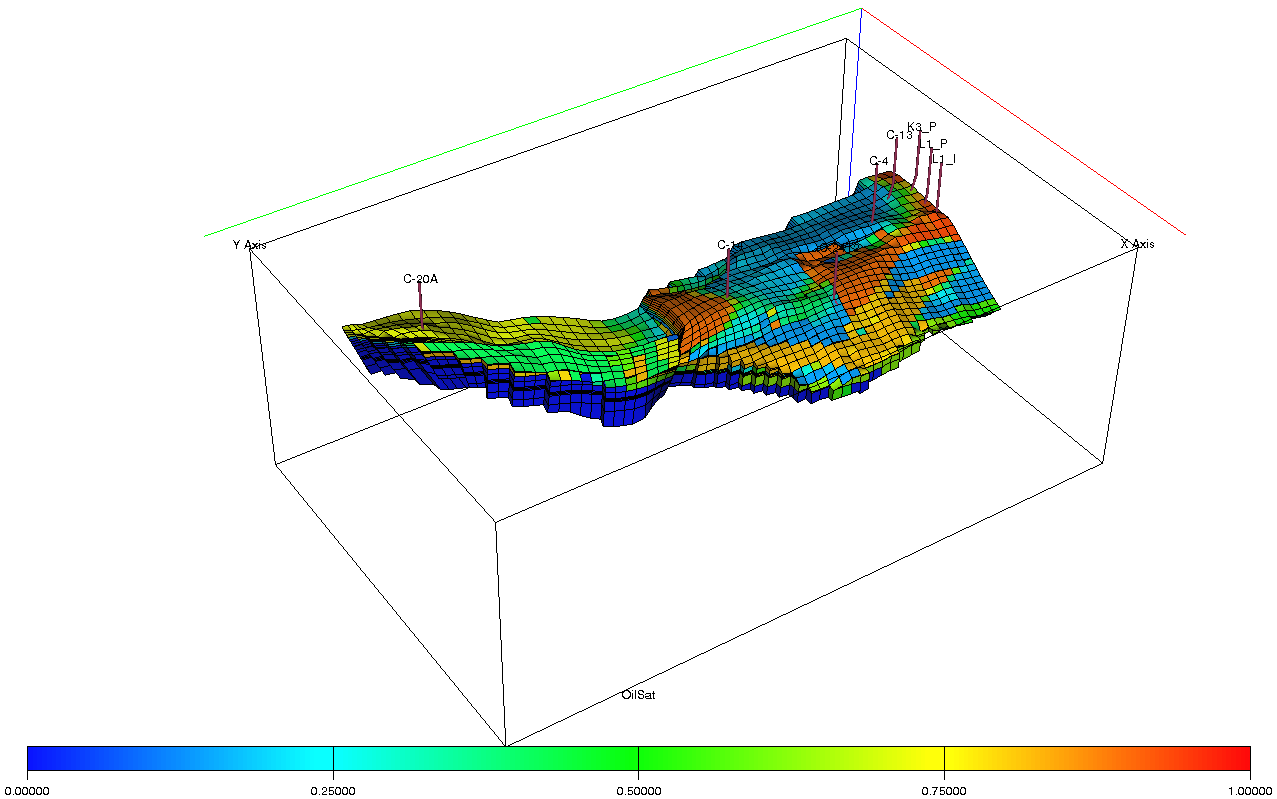
\includegraphics[width=\textwidth]{reservoir}
  \caption{Example of a reservoir, visualization is done with floviz software.}
  \label{floviz}
\end{figure}


\begin{itemize}
  \item
  \item Factorization have little data reuse
  \item Solve don't have data reuse
  \item Facto time, aggregation improve speed-up but less than domain decomposition
  \item Solve time, same as facto
  \item Agg time, need to be considerate, could be avoid by many facto/solve or compute offline if possible
  \item We have a data locality problem and task aren't big enough
  \item benefit of task scheduling in load balancing
\end{itemize}

\subsection{Generality}
Reservoir simulation is a software used by petroleum company to be able to optimize oil recovery.
%
For example, reservoir engineer can use reservoir simulation to identifying a good location for wells.
%
It is also used to forecast oil production


\subsection{From physical equations to linear system}
To be able to do reservoir simulation, we start with a physicist who model fluid flow inside porous medium.
%
From this model, we can obtain some physical equations.
%
Then we discretize the reservoir into cells and we use a finite difference schema.
%
For each cell of the reservoir, we can compute a non-linear equation of each variables (e.g.: pressure, oil saturation)
%
To solve the non-linear systems of equation, we use the Newton–Raphson method.
%
This method is iterative, we begins with an initial guess $X_0$ reasonably close to the solution $X_n$ which satisfied $F(X_n) = 0$.

%   (-_-)   %
\begin{figure}[!ht]
  \centering
  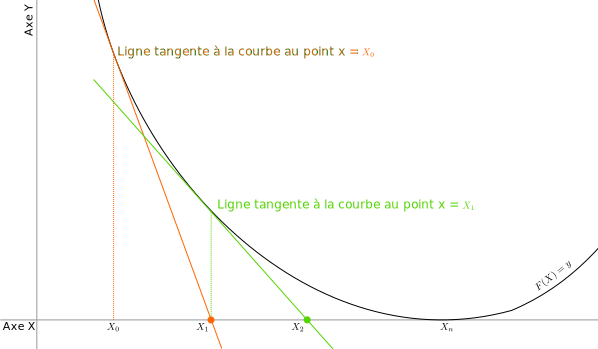
\includegraphics[width=\textwidth]{newton}
  \caption{Example of two Newton steps in one dimension space.
    Each tangent lines correspond to a linear equation to solve.}
  \label{newton}
\end{figure}

The example in the figure~\ref{newton} is only in one dimension but it's quite the same approach that can be done when we work with an arbitrary number of dimensions.


\subsection{Solving the linear system}
A popular approach to solve large sparse linear systems of equation is a Krylov
method (like GMRES or Conjugate Gradient) preconditioned by an incomplete
factorization (see~\cite{Saad96IMSLS}).
%
This is often the most time consuming part of a numerical simulation.
%
In this method there is two major operations, the first step is the {\em ILU matrix factorization}
and the second step is the {\em triangular solve}.
%The usual way to parallelize those kind of solver is to use a weaker form of
%the preconditioner in parallel by preconditioning subdiagonal block of the
%matrix: the subdiagonal block are usually obtained thank to a partition of
%the adjacency graph of the matrix.
Outside the preconditioner, the operations required in a Krylov method are
mostly BLAS1 operations and matrix vector products which naturally dealt with
parallel loop splitting.
In our experiments, we focus on the fine grain parallelization of
the ILU preconditioner; that is to say the factorization of the matrix (done once per system solve) and
the triangular system solves (done once at each iteration of the system solve).


Both of those algorithms (factorization and triangular solve) can naturally be represented as a task graph. For example in the factorization
a task corresponds to the factorization of a matrix row and the dependencies are directly given by the non-zero pattern of the matrix.
%Indeed, the factorization of row $i$ can be done only when all the rows which index corresponds to an entry in the non-zero array of row $i$ before the diagonal have been factorized.
Indeed, to factorize the row $i$, we need to factorize all the rows $j$ lower than $i$
% which have an entry in the non-zero array of row $i$.
such that the entry $(i,j)$ is non-zero.
Therefore the DAG description is easily built from the non-zero pattern of the matrix:
the task $i$ corresponds to row $i$ of the matrix, the predecessor tasks of task $i$ are given by the column index of non-zero coefficients before the diagonal in row $i$
 and successor tasks of task $i$ are given by the row index of non-zero coefficients below the diagonal in the column $i$.

Incomplete factorization and associated triangular solve of a sparse matrix
is a problem that is well representative of the difficulty that one can encounter
with fine-grain parallelization: The fine grain description of these algorithms
is natural, but in practice, a straightforward task based parallelization using TBB or
OpenMP does not deliver good speed-ups because of the very low computational cost of
a task and the NUMA effect when accessing the coefficient of the matrix and vector.
In the experiment results, we will evaluate our programming model on those algorithms.


We perform the tests on two linear systems. The first one, Cube\_100, is a
system obtained from a 7 points discretization scheme (e.g., finite volume) of regular
3D cubes with 100 points along each dimension.
It is a scalar system; each row of the matrix is a vector of coefficients stored in double precision.
The second one, SPE10, corresponds to a 7 points discretization of a reference problem from petroleum industry~\cite{spe10}.
In this case each entry of the matrix is a small dense block $(3,3)$ of coefficients stored in double precision.
Due to the geometry of the problem, for Cube\_100, the task dependency graph is very regular whereas it is an irregular one in the SPE10 case.
The characteristics of the matrices are listed in Table~\ref{matrices}.

\begin{table}[!h]
  \renewcommand{\arraystretch}{1.3}
  \caption{Matrices used in tests.}
  \label{matrices}
  \centering
  \begin{tabular}{|c||c|c|}
    \hline
    Name & Cube\_100 & SPE10\\
    \hline
    \hline
%    Type & Synthetic & Real Life Case\\
%    \hline
    Rows ($n$) & 1,000,000 & 3,283,263\\
    \hline
    Number of non-zeros ($nnz$) & 6,940,000 & 67,303,269\\
    \hline
    Entries of the matrix & Scalars & $(3,3)$ dense blocks\\
    \hline
  \end{tabular}
\end{table}

Each fine grain task performs one elementary line operation. SPE10
tasks weight 2-5 times more than Cube\_100 tasks. However, both
cases generate approximately 1 million tasks each.

The test protocol is the following:
\begin{itemize}
\item Each test is run three times, the final retained result is
  computed as the average of the three measured results. For each
  test, we collect three different timings:
  factorization time, triangular solve time, and aggregation time.

\item We perform the tests on a single socket (using
      {\em numactl --cpunodebind}) and on two sockets.

  % OA: je pense qu'un mot d'explication sur l'ordering sera
  % necessaire

\item We test two orderings (set of row/column permutations): A {\em natural} ordering which corresponds to no
      modification on matrix structure where unknowns are sequentially
      ordered by plane along the geometric z axis
      (this leads to a perfect seven diagonals pattern for Cube\_100)
      and a {\em nested dissection}~\cite{Saad96IMSLS} ordering which exposes more parallelism.

  % ST: TODO: expliquer brièvement ce que sont les natural et nest
  % dissection orderings.
  % ST: TODO: expliquer pourquoi ça n'a pas de sens d'appliquer
  % D() au cas nested dissection.

\item We test three levels of ILU(k) fill: 0, 1 and 2.
      The level $k$ of ILU(k) preconditioner determines the level of fill of
      the matrix. In others words, computation per line and the number of dependencies
      between tasks grow up with a greater $k$. Table~\ref{tab:edges} gives the number of edges resulting in the DAG of the factorization
      (triangular solve DAG has a similar number of edges) for ILU$(0)$, ILU$(1)$ and ILU$(2)$. Subsection \ref{precond_step} will also give some features on the cost of a computational task (one row factorization)
      depending on the ILU level of fill parameter.

\item For the parameterized aggregation heuristics, we select the
      parameter values leading to the best performance result. With
      natural ordering, we can use the Cache Oriented algorithm because of
      particular DAG structure. With nested dissection ordering, the Cache Oriented algorithm
      can't be used, so we use the Depth Front algorithm with a high value.
\end{itemize}



%-------------------------------
\subsection{ILU(k) Factorization Step}
\label{precond_step}
The first test series is performed on the ILU(k) factorization step
on a single 4-core socket (Tables~\ref{tab:tbb:4:facto:no},~\ref{tab:tbb:4:facto:nested}).

% ST: TODO: mentionner que ça consiste ici en trois phases de
% préconditionnement: ILU(0), ILU(1), ILU(2), et indiquer brièvement la
% différence entre ces phases. Tout le monde ne connait pas
% GMRES, loin de là:)
With aggregation disabled the task-parallel ILU(0) factorization is always
slower than the sequential version. This is due to the additional cost
of task management. Tasks duration for CUBE\_100 in ILU(0) is only $50\,ns$ and
$240\,ns$ for SPE10, but one task
management duration is approximately $500\,ns$. In ILU(2), tasks are bigger, their
duration is $600\,ns$ for CUBE\_100 and $1.7\,\mu{s}$ for SPE10 but it's
not bigger enough to consider task management negligible.
Another important aspect of the ILU factorization and triangular solve is that on our testbed machine
the algorithm speed-up is bounded by the memory bandwidth: Therefore the maximum theoretical speed-up achievable
by such algorithms on several cores is less than the number of cores used.

With aggregation enabled and {\em CD(4)} coarse strategy string, we now reduce the number
of tasks to 2,500 with a task duration 400 times bigger.
In ILU(0) we achieve a moderate speed-up of 2. ILU(2) factorization achieves a
better speed-up of 3. The Front algorithm is not as effective as
the Depth Front in this test case, because it doesn't aggregate tasks
with continuous lines, which cause many cache misses.

% ST: TODO: Que veut dire contiguous data?
% ST: TODO: est-ce que ça aide de faire plusieurs D(4) ? En faire
% plus aurait-il aidé plus ? Discuter de quand s'arrêter ?

With the Front algorithm ({\em F(32)}) in ILU(0) with natural ordering,
%tasks at the begin and the end of the DAGs are not aggregated,
we aggregate a maximum of 157 tasks together and, on average, we aggregate only 53 tasks.



\begin{table}[!h]
  \renewcommand{\arraystretch}{1.3}
  \caption{Results on the ILU(k) factorization step on a single 4-core
    socket with TBB with nested dissection ordering.}
  \label{tab:tbb:4:facto:nested}
  \centering
  \begin{tabular}{|c|c||c|c|c|c|}
    \hline
    Matrix & ILU & Sequential & No agg. & F(32) & D(400)\\
    &     &  (second)  & \multicolumn{3}{c|}{(speed-up)}\\
    \hline
    \hline
    & ILU(0) & 0.129 & 0.46 & 2.17 & 2.26\\
    CUBE\_100 & ILU(1) & 0.495 & 1.29 & 1.70 & 2.78\\
    & ILU(2) & 0.828 & 1.74 & 1.94 & {\bf 3.12}\\
    \hline
    & ILU(0) & 0.276 & 0.74 & 1.93 & 2.16\\
    SPE10     & ILU(1) & 1.375 & 1.98 & 1.67 & 2.82\\
    & ILU(2) & 2.247 & 2.43 & 1.85 & {\bf 3.12}\\
    \hline
  \end{tabular}
\end{table}

With two 4-core sockets (Tables~\ref{tab:tbb:8:facto:no},~\ref{tab:tbb:8:facto:nested}), the parallel
ILU(0) again performs slower than sequential execution when
aggregation is disabled. With aggregation enabled, the ILU(0)
achieves a speed-up of 3. ILU(2) achieves a speed-up of 6.2.

\begin{table}[!h]
  \renewcommand{\arraystretch}{1.3}
  \caption{Results on the ILU(k) factorization step on two 4-core
    sockets with TBB with natural ordering.}
  \label{tab:tbb:8:facto:no}
  \centering
  \begin{tabular}{|c|c||c|c|c|c|}
    \hline
    Matrix & ILU & Sequential & No agg. & F(32) & CD(4)\\
    &     &  (second)  & \multicolumn{3}{c|}{(speed-up)}\\
    \hline
    \hline
    \hline
    & ILU(0) & 0.056 & 0.28 & 1.27 & 2.54\\
    CUBE\_100 & ILU(1) & 0.143 & 0.65 & 1.89 & 3.79\\
    & ILU(2) & 0.612 & 1.47 & 3.06 & 3.91\\
    \hline
    & ILU(0) & 0.260 & 0.97 & 2.48 & 3.78\\
    SPE10     & ILU(1) & 0.771 & 2.24 & 3.80 & 5.72\\
    & ILU(2) & 2.006 & 3.37 & 3.97 & {\bf 6.21}\\
    \hline
  \end{tabular}
\end{table}


\begin{table}[!h]
  \renewcommand{\arraystretch}{1.3}
  \caption{Results on the ILU(k) factorization step on two 4-core
    sockets with TBB with nested dissection ordering.}
  \label{tab:tbb:8:facto:nested}
  \centering
  \begin{tabular}{|c|c||c|c|c|c|}
    \hline
    Matrix & ILU & Sequential & No agg. & F(32) & D(400)\\
    &     &  (second)  & \multicolumn{3}{c|}{(speed-up)}\\
    \hline
    \hline
    & ILU(0) & 0.127 & 0.41 & 3.10 & 3.31\\
    CUBE\_100 & ILU(1) & 0.483 & 1.31 & 2.70 & 4.77\\
    & ILU(2) & 0.817 & 1.96 & 3.18 & 5.46\\
    \hline
    & ILU(0) & 0.277 & 0.71 & 2.59 & 3.09\\
    SPE10     & ILU(1) & 1.452 & 2.48 & 2.81 & 5.00\\
    & ILU(2) & 2.347 & 3.29 & 3.12 & {\bf 5.57}\\
    \hline
  \end{tabular}
\end{table}

%-------------------------------
\subsection{Triangular Solve Step}\label{subsec:solve}

The triangular solve step is itself composed of two parts: A
{\em forward} substitution followed by a {\em backward}
substitution. The DAG of the forward substitution is identical to
the DAG of the factorization step mentioned in the previous section.
Thus we can reuse the same coarse
DAG. In our test cases, the DAG of the backward substitution part is
the transpose of the DAG of the forward substitution. Here again,
the factorization coarse DAG can thus straightforwardly be reused.
In total we have twice more tasks in triangular solve than in factorization.

The weight of operations done in triangular solve elementary tasks
is lighter than their factorization task counterparts.
%% and these tasks need to access to more data..
Tests on a
single 4-core socket (Tables~\ref{tab:tbb:4:solve:no},~\ref{tab:tbb:4:solve:nested})
show that the parallel triangular solve is always slower than
the sequential version with task aggregation disabled. With
aggregation enabled, we obtain a speedup of~2.

% ST: TODO: idéalement il faudrait que ces deux tables se retrouvent
% côte à côte dans la version finale.
\begin{table}[!h]
  \renewcommand{\arraystretch}{1.3}
  \caption{Results on the Triangular Solve step on a single 4-core
    socket with TBB with natural ordering.}
  \label{tab:tbb:4:solve:no}
  \centering
  \begin{tabular}{|c|c||c|c|c|c|}
    \hline
    Matrix & ILU & Sequential & No agg. & F(32) & CD(4)\\
    &     &  (second)  & \multicolumn{3}{c|}{(speed-up)}\\
    \hline
    \hline
    & ILU(0) & 0.092 & 0.23 & 0.88 & 1.90\\
    CUBE\_100 & ILU(1) & 0.117 & 0.27 & 0.82 & 1.97\\
    & ILU(2) & 0.163 & 0.34 & 0.92 & 2.05\\
    \hline
    & ILU(0) & 0.219 & 0.40 & 1.08 & 1.93\\
    SPE10     & ILU(1) & 0.353 & 0.62 & 1.37 & 2.22\\
    & ILU(2) & 0.554 & 0.85 & 1.58 & {\bf 2.39}\\
    \hline
  \end{tabular}
\end{table}

\begin{table}[!h]
  \renewcommand{\arraystretch}{1.3}
  \caption{Results of the Triangular Solve step on a single 4-core
    socket with TBB with nested dissection ordering.}
  \label{tab:tbb:4:solve:nested}
  \centering
  \begin{tabular}{|c|c||c|c|c|c|}
    \hline
    Matrix & ILU & Sequential & No agg. & F(32) & D(400)\\
    &     &  (second)  & \multicolumn{3}{c|}{(speed-up)}\\
    \hline
    \hline
    & ILU(0) & 0.107 & 0.20 & 1.19 & 1.34\\
    CUBE\_100 & ILU(1) & 0.150 & 0.31 & 0.94 & 1.39\\
    & ILU(2) & 0.171 & 0.34 & 0.95 & 1.50\\
    \hline
    & ILU(0) & 0.249 & 0.37 & 1.39 & 1.52\\
    SPE10     & ILU(1) & 0.430 & 0.65 & 1.32 & 1.77\\
    & ILU(2) & 0.500 & 0.72 & 1.35 & {\bf 1.89}\\
    \hline
  \end{tabular}
\end{table}

On two 4-core sockets
(Tables~\ref{tab:tbb:8:solve:no},~\ref{tab:tbb:8:solve:nested}), with
task aggregation disabled, only the SPE10 test achieves a speedup
greater than 1. With aggregation enabled, a speedup of 2.52 is
achieved on ILU(0) and a speedup of 4.14 is achieved on ILU(2).

\begin{table}[!h]
  \renewcommand{\arraystretch}{1.3}
  \caption{Results of the Triangular Solve step on two 4-core sockets with
    TBB with natural ordering.}
  \label{tab:tbb:8:solve:no}
  \centering
  \begin{tabular}{|c|c||c|c|c|c|}
    \hline
    Matrix & ILU & Sequential & No agg. & F(32) & CD(4)\\
    &     &  (second)  & \multicolumn{3}{c|}{(speed-up)}\\
    \hline
    \hline
    & ILU(0) & 0.092 & 0.27 & 1.27 & 2.44\\
    CUBE\_100 & ILU(1) & 0.123 & 0.35 & 1.54 & 2.82\\
    & ILU(2) & 0.174 & 0.45 & 1.40 & 2.98\\
    \hline
    & ILU(0) & 0.219 & 0.53 & 1.63 & {\bf 2.52}\\
    SPE10     & ILU(1) & 0.408 & 0.96 & 2.39 & 3.77\\
    & ILU(2) & 0.658 & 1.38 & 2.79 & {\bf 4.14}\\
    \hline
  \end{tabular}
\end{table}


\begin{table}[!h]
  \renewcommand{\arraystretch}{1.3}
  \caption{Results of the Triangular Solve step on two 4-core
    sockets with TBB with nested dissection ordering.}
  \label{tab:tbb:8:solve:nested}
  \centering
  \begin{tabular}{|c|c||c|c|c|c|}
    \hline
    Matrix & ILU & Sequential & No agg. & F(32) & D(400)\\
    &     &  (second)  & \multicolumn{3}{c|}{(speed-up)}\\
    \hline
    \hline
    & ILU(0) & 0.107 & 0.18 & 1.41 & 1.67\\
    CUBE\_100 & ILU(1) & 0.156 & 0.32 & 1.36 & 1.92\\
    & ILU(2) & 0.180 & 0.36 & 1.37 & 2.08\\
    \hline
    & ILU(0) & 0.249 & 0.35 & 1.64 & 1.82\\
    SPE10     & ILU(1) & 0.496 & 0.80 & 2.12 & 2.71\\
    & ILU(2) & 0.578 & 0.90 & 2.19 & {\bf 2.90}\\
    \hline
  \end{tabular}
\end{table}

% In most cases, domain decomposition achieves better raw performance
% results. However, by avoiding potentially harmful domain boundaries artifacts, the
% aggregation method ensures a better overall numerical stability than the
% domain decomposition.
